\chapter{Equazioni differenziali ordinarie}
\section{Introduzione alle \odes}
\begin{definition} \label{Def: ODE}
Si dice \textbf{equazione differenziale ordinaria} di ordine $n$ un'equazione funzionale della forma
\begin{equation}
    F\left(x, y(x), y'(x), \dots, y^{(n)}(x)\right)=0
\end{equation}
dove  $F:A \subseteq \R^{n+2} \to \R$, $y=y(x)$ è l'incognita e $x$ è la variabile indipendente.
\end{definition}
\begin{oss}
    Solitamente $F$ è una funzione continua.
\end{oss}
\begin{oss}
    È abbastanza frequente l'omissione della variabile indipendente nella scrittura dell'equazione.
\end{oss}
\begin{definition} \label{Def: ODE in forma normale}
    Un'\ode si dice in \textbf{forma normale} se è del tipo
    \begin{equation}
        y^{(n)}(x)=f\left(x, y(x), y'(x), \dots, y^{(n-1)}(x)\right)
    \end{equation}
    con $f:A\subseteq \R^{n+1} \to \R$, $A$ aperto.
\end{definition}
\begin{definition} \label{Def: Soluzione di un'ode}
    Si dice \textbf{soluzione} o \textbf{integrale} dell'\ode su un certo $I\subseteq \R$ una funzione $\varphi: I \to \R$ derivabile $n$ volte su $I$ tale che 
    \begin{equation}
         F\left(x, \varphi(x), \varphi'(x), \dots, \varphi^{(n)}(x)\right)=0 \qquad \forall\ x \in I
    \end{equation}
\end{definition}
\begin{example}
    Si prenda la seguente equazione in forma normale di ordine 1: 
    \begin{equation*}
        y'(x)=y(x)
    \end{equation*}
    Essa è verificata in ogni $x \in \R$ dalla funzione $\varphi(x)= e^x$.
\end{example}
Oltre a parlare di equazioni differenziali ordinarie, si può parlare di sistemi di equazioni differenziali ordinarie di ordine $n$.
\begin{definition} \label{Def: Sistema di ode del primo ordine}
    Si dice \textbf{sistema di \odes del primo ordine} un sistema di equazioni del tipo
    \begin{equation}
        \left\{
        \begin{aligned}
        y_1'(x) &= f_1(x, y_1, \dots, y_n)\\
         y_2'(x) &= f_2(x, y_1, \dots, y_n)\\       
        &\vdots \\
        y_n'(x) &= f_n(x, y_1, \dots, y_n)
        \end{aligned} \right.
\end{equation}
o, in forma compatta, 
\begin{equation}
    Y'=G(x, Y)
\end{equation}
con $Y: I \subseteq \R \to \R^n,\ Y=(y_1, \dots, y_n)$ e $G:I \times \R^n \to \R^n,\ G(x, Y)=(f_1, \dots, f_n)$
\end{definition}
\begin{definition} \label{Def: Sistema di ode lineare}
    Un sistema di \odes del primo ordine si dice \textbf{lineare} se $G$ è lineare in $Y$.
\end{definition}
\begin{definition} \label{Def: Sistema/Ode autonoma}
    Un sistema di \odes del primo ordine o un'\ode di ordine $n$ si dicono \textbf{autonomi} se non è presente una dipendenza esplicita da x, cioè se $G=G(y)$.
\end{definition}
\begin{lemma} \label{Lemma: Equivalenza equazione-sistema}
    Un'\ode di ordine $n$ in forma normale è equivalente ad un sistema di \odes del primo ordine in $\R^n$.
\end{lemma}
\begin{proof}
    Sia
    \begin{equation}
  (E):\ y^{(n)}=f\left(x, y(x), y'(x), \dots, y^{(n-1)}(x)\right)
    \end{equation}
    e si costruisca il vettore $Y=(Y_1, \dots, Y_n)$ come segue: 
    \begin{equation}
        \begin{aligned}
        Y_1(x)&:= \overline{y}(x)\\
        Y_2(x)&:= \overline{y}'(x)\\
            &\vdots\\
        Y_n(x)&:= \overline{y}^{(n-1)}(x)
        \end{aligned}
    \end{equation}
    Si può osservare che,
    \begin{equation}
      (S):\ Y'= \begin{cases}
            Y_1'&= Y_2\\
            Y_2'&=Y_3\\
            &\vdots\\
            Y_n'&= \left(\overline{y}^{(n-1)}\right)'=\overline{y}^{(n)}
        \end{cases}
    \end{equation}
    Definendo poi
    \begin{equation}
        G(x, Y) := \begin{pmatrix}
            y_1\\
            y_2\\
            \vdots\\
            f(x, y_1, \dots, y_n)
        \end{pmatrix}
    \end{equation}
    Si ha che, se $\overline{y}$ soddisfa $E$, allora $Y(x)$
    soddisfa $Y'=G(x, Y)$. D'altra parte, se $Y$ soddisfa $Y'=G(x, Y)$, la sua prima componente $y_1(=\overline{y}(x))$ soddisfa $E$.
\end{proof}
\begin{oss}
Un'\ode ha generalmente infinite soluzioni. Infatti, dette $g, G$ rispettivamente una funzione generica e una sua primitiva, si ha che
\begin{equation}
    y'= g(x) \Rightarrow y(x)= G(x)+c,\quad c \in \R
\end{equation}
\end{oss}
\section{Problema di Cauchy}
\begin{definition}
    Si dice \textbf{problema di Cauchy} associato ad un sistema S: Y'=G(x,Y) il sistema
    \begin{equation}
       (P): \begin{cases}
            Y'=G(x, Y)\\
            Y(x_0)=Y_0
        \end{cases}
    \end{equation}
    dove $Y(x_0)$ è detto \textbf{condizione iniziale}.
\end{definition}
\begin{oss}
In un problema del genere è necessario che $x_0 \in \R,\ y_0 \in \R^n$ siano noti.
\end{oss}
\begin{lemma}[Formulazione integrale del problema di Cauchy] \label{Lemma: Formulazione integrale del problema di Cauchy}
    Sia $f: A \subseteq \R^{n+1} \to \R^n$, $A$ aperto, $f \in C^0(A)$. Sia $(x_0, y_0) \in A$. Allora le seguenti affermazioni sono equivalenti
    \begin{enumerate}
        \item Esiste $y=y(x)$ derivabile in $[x_0-\delta, x_0+\delta],\ \delta>0$ tale che 
        \begin{equation}
            (P): \begin{cases}
                y'(x)=f(x, y(x)) \qquad (E)\\
                y(x_0)=y_0 
            \end{cases}
            \qquad \forall\ x \in [x_0-\delta, x_0+\delta]
        \end{equation}
        \item Esiste $y=y(x)$ continua in $[x_0-\delta, x_0+\delta],\ \delta>0$ tale che 
        \begin{equation} \label{Eq: Equazione integrale di Volterra}
            y(x)= y_0 + \int\limits_{x_0}^{x}{f(s, y(s))}\, ds \qquad \forall\ x \in [x_0-\delta, x_0+\delta]
        \end{equation}
    \end{enumerate}
\end{lemma}
\begin{proof}
    $1 \Rightarrow 2$: Sia $y$ come nelle ipotesi di $(1)$. Si integrino entrambi i membri di $(E)$ tra $x_0$ e $x \in [x_0-\delta, x_0+\delta]$. Allora
    \begin{equation}
        y(x)-y_0=\int\limits_{x_0}^{x}{f(s, y(s))}\,ds
    \end{equation}
    e $y$ è continua e soddisfa $(2)$.\\
    $2 \Rightarrow 1$: Sia $y$ come nelle ipotesi di $(2)$. Allora si ha che
    \begin{equation}
        y(x_0)= y_0 + \int\limits_{x_0}^{x_0}{f(s, y(s))}\, ds= y_0
    \end{equation}
    Poi, $f(s, y(s))$ è continua per composizione di funzioni $C^0$. Quindi dal TFC, $y(x)$ è derivabile e
    \begin{equation}
        y'(x)= \left[y_0 + \int\limits_{x_0}^{x}{f(s, y(s))}\, ds\right]'= f(x, y(x)) \qquad \forall\ x \in [x_0-\delta, x_0+\delta]
    \end{equation}
    cioè che $y$ risolve il problema (P) di Cauchy.
\end{proof}
\begin{theorem}[Teorema di Peano dell'esistenza locale]
Si consideri il problema di Cauchy
\begin{equation}
    (P): \begin{cases}
        Y'=G(x, Y)\\
        Y(x_0)=Y_0
    \end{cases}
\end{equation}
Se $G \in C^0(B_\delta(x_0, y_0))$, allora esistono $\delta>0,\ \varphi$ tali che $\varphi: (x_0- \delta, x_0+\delta) \to \R^n$ sia soluzione di P.
\end{theorem}
Il teorema garantisce l'esistenza della soluzione ma non l'unicità.
\begin{example}
Si consideri il seguente problema di Cauchy.
\begin{equation*}
    (P):\begin{cases}
        y'=3y^{\frac{2}{3}}\\
        y(0)=0
    \end{cases}
\end{equation*}
Si può facilmente osservare che la soluzione costante $y=0$ è una soluzione del problema.\\
Un'altra soluzione può essere $y=x^3$, infatti
\begin{equation*}
    y(0)=0^3=0, \qquad y'(x)=3x^2=3(x^3)^\frac{2}{3}=3x^2
\end{equation*}
Allo stesso modo, si può mostrare che, fissati $a,\ b \in \R$ tali che $a<0<b$, la funzione
\begin{equation*}
y^*= \begin{cases}
    (x-a)^3 &\qquad x\leq a\\
    0 &\qquad a \leq x \leq b\\
    (x-b)^3 &\qquad x \geq b
\end{cases}
\end{equation*}
è anch'essa soluzione del problema di Cauchy.\\
Pertanto, le soluzioni del problema sono infinite e una loro rappresentazione grafica dà vita al cosiddetto \textit{pennello di Peano}.
\begin{figure}[H]
\centering
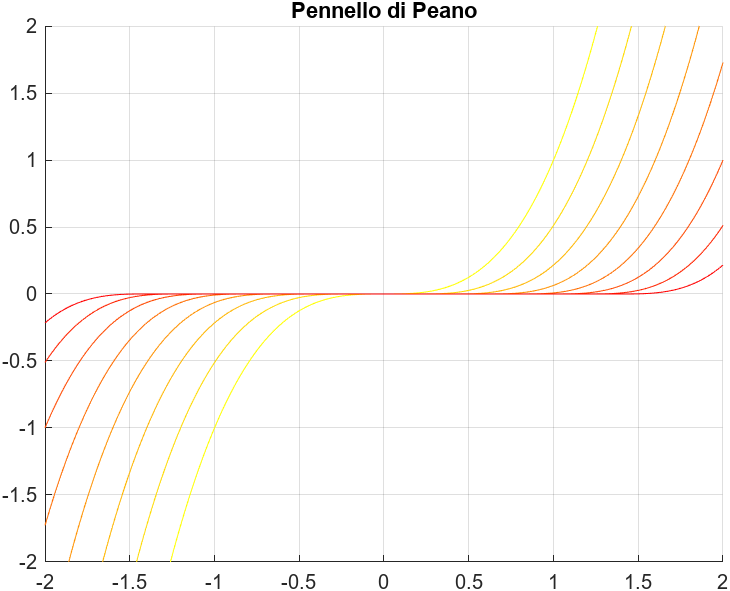
\includegraphics[width=0.31\textwidth]{Capitoli/Capitolo8/Pennello di Peano.png}
\end{figure}
\end{example}
È altresì possibile stabilire una condizione sufficiente per l'esistenza e unicità locale di un problema di Cauchy. Prima però bisogna definire il concetto di lipschitzianità locale (\ref{Def: Funzione lipschitziana}).
\begin{definition}
    Si dice che una funzione $G: A\subseteq \R^{n+1} \to \R^n$ con $A$ aperto è \textbf{localmente Lipschitziana} nell'insieme $A$ in $y$ uniformemente rispetto a $x$ se in ogni compatto $K \subset A$ esiste una costante di Lipschitz $L_K$ tale che
    \begin{equation}
        \forall\ (x, y_1), (x, y_2) \in K \ \text{si ha che}\ |G(x, y_1)-G(x, y_2)| \leq L_K |y_1-y_2|
    \end{equation}
\end{definition}
\begin{theorem}[Teorema di Cauchy di esistenza e unicità locale] \label{Teo: Esistenza e unicità locale}
    Siano $A \subseteq \R^{n+1}$ aperto e $G:A \to \R^n$ continua, localmente Lipschitziana in $Y$ e uniformemente rispetto a $x$ in $B_\delta(x_0, y_0) \subset A$. Sia poi $(x_0, Y_0) \in A$. Allora esiste $\delta>0$ tale che il problema di Cauchy
    \begin{equation}
        (P): \begin{cases}
            Y'=G(x, Y)\\
            Y(x_0)=Y_0
        \end{cases}
    \end{equation}
    ammetta un'unica soluzione locale $\overline{Y}$ per $x \in [x_0-\delta, x_0+\delta]$
\end{theorem}
\begin{proof}
Siano $a, b>0$ tali che si possa definire $R \subseteq A$ come
\begin{equation}
    R= \{(x,y) \mid |x-x_0|\leq a, |y-y_0| \leq b \}
\end{equation}
Siano poi $L>0$ la costante di Lipschitz di $G$ su $R$ e 
\begin{equation}
M=\max\limits_{R}{|G(x, y)|} \qquad 0<\delta<\min\left\{a, \frac{b}{M}, \frac{1}{L}\right\}
\end{equation}
Dopodiché, definito $B$ come
\begin{equation}
    B=\{y \in C^0([x_0-\delta, x_0+\delta]) \mid d_\infty(y, y_0) \leq b\} \subset (C^0([x_0-\delta, x_0+\delta]), d_\infty)
\end{equation}
si mostri che esso è chiuso ($\Rightarrow$ $B$ completo per \ref{Teo: Sottospazio chiuso di un completo è completo}).
Perciò, si consideri una successione $\{y_k\}_k \subset B$ tale che $y_k \to \overline{y}$ rispetto a $d_\infty$. Affinché $B$ sia completo, occorre che $\overline{y} \in B$, cioè $d_\infty(\overline{y},y_0)\leq b$, dunque
\begin{equation}
    d_\infty(\overline{y},y_0) \leq d_\infty(\overline{y},y_k)+ d_\infty(y_k,y_0) \leq d_\infty(\overline{y},y_k) +b
\end{equation}
Allora, passando al limite per $k \to +\infty$ si ha che
\begin{equation}
    d_\infty(\overline{y},y_0) \leq \lim_{k \to +\infty}{d_\infty(\overline{y},y_k) +b}= 0+b= b
\end{equation}
cioè $\overline{y} \in B$, quindi $(B, d_\infty)$ è uno spazio metrico completo.\\
A questo punto, si definisca la mappa $H$
\begin{equation}
    \begin{aligned}
        H: B &\to B\\
        y &\mapsto z:=H(y)
    \end{aligned}
\end{equation}
con
\begin{equation}
    z(x)=y_0+ \int\limits_{x_0}^{x}{G(s, y(s))}\,ds
\end{equation}
Si verifichi che $H$ sia ben definita, cioè che $H(y)$ è continua e che, se $y \in B$, allora $H(y)=z \in B$. Chiaramente $z \in C^0([x_0-\delta, x_0+\delta])$. Inoltre,
\begin{equation}
    |z(x)-y_0|=\left|\int\limits_{x_0}^{x}{G(s, y(s))}\,ds\right| \leq
\int\limits_{x_0}^{x}\left|{G(s, y(s))}\right|\,ds
\end{equation}
Poiché $y \in B$, per ogni $s$ si ha $|y(s)-y_0|\leq b$. Dalla definizione di $\delta$ si ricava che $|s-x_0|<\delta<a$. Perciò $(s, y(s)) \in R$. In particolare, vale anche che $G(s, y(s)) \leq M$. Per definizione di $\delta$, allora,
\begin{equation}
    |z(x)-y_0|\leq M|x-x_0|\leq M\delta \leq b \qquad \forall\ x \in [x_0-\delta, x_0+\delta]
\end{equation}
cioè $H(y) \in B$.\\
Si mostri poi che $H$ è una contrazione. Siano $y_1, y_2 \in B$.
\begin{equation}
\begin{aligned}
    d_\infty(H(y_1), H(y_2))&= \sup_{x \in [x_0-\delta, x_0+\delta]}{|H(y_1)(x)-H(y_2)(x)|}=\\
    &=\sup_{x \in [x_0-\delta, x_0+\delta]}\left|{\int\limits_{x_0}^{x}{\left[G(s,y_1(s))-G(s, y_2(s))\right]}}\,ds\right| \leq \\
    &\leq \sup_{x \in [x_0-\delta, x_0+\delta]}{\int\limits_{x_0}^{x}{\left|G(s,y_1(s))-G(s, y_2(s))\right|}}\,ds \leq\\
    &\leq L\,  \sup_{x \in [x_0-\delta, x_0+\delta]}{\int\limits_{x_0}^{x}{\left|y_1(s)-y_2(s)\right|}}\,ds\leq\\
    &\leq L \,d_\infty(y_1, y_2)\, |x-x_0| \\
    &\leq L\, \delta\, d_\infty(y_1, y_2) \leq \gamma\, d_\infty(y_1,y_2)
\end{aligned}
\end{equation}
dove $\gamma<1$ poiché $\delta<\tfrac{1}{L}$. Dunque $H$ è una contrazione e, per il teorema delle contrazioni \eqref{Teo: delle contrazioni}, esiste un solo punto fisso $y$ tale che
\begin{equation}
    y=H(y)=z= y_0+ \int\limits_{x_0}^{x}{G(s, y(s))}\,ds
\end{equation}
che risolve il problema di Cauchy per il lemma \ref{Lemma: Formulazione integrale del problema di Cauchy}.
\end{proof}
\begin{oss}
    Si noti che una funzione $C^1(A)$ è ivi localmente Lipschitziana, perciò  è sufficiente la regolarità del secondo membro per poter applicare il teorema di Cauchy.
\end{oss}
\begin{example}
    Si riprenda il problema di prima ma si modifichi la condizione iniziale.
    \begin{equation*}
        P: \begin{cases}
        y'=3y^{\frac{2}{3}}\\
        y(0)=3
    \end{cases}
    \end{equation*}
    In questo caso la funzione è $C^\infty(B_\delta(0,3))$, dunque vale il teorema di Cauchy e la soluzione è unica.
\end{example}
\begin{definition} \label{Prolungamento}
    Sia $y(x)$ una soluzione dell'equazione $(E):\ y'=f(x,y)$ definita su $(a,b)$. Si dice che $y_1$ è un \textbf{prolungamento} di $y$ se $y_1(x)$ è una soluzione di $(E)$, è definita su $(a_1, b_1) \supset (a,b)$ e coincide con $y$ in $(a,b)$.\\
    Inoltre, un prolungamento $y_1(x)$ di $y(x)$ si dice \textbf{massimale} se per ogni prolungamento $y_2(x)$ di $y(x)$ definito su $(a_2, b_2)$ si ha che $(a_2, b_2) \subset (a_1, b_1)$.
\end{definition}
\begin{oss}
Data tale definizione, può aver senso ragionare sull'unicità del prolungamento. Perciò, ci si ponga nelle ipotesi del teorema di esistenza e unicità locale. Dopodiché siano $y_1,\ y_2 : (a,b) \to \R$ soluzioni tali che $y_1(x_0)=y_2(x_0)$ e si mostri che non esiste $x_1 \in (a,b)$ tale che $y_1(x_1) \neq y_2(x_1)$. Difatti, se $y_1 \not\equiv y_2$ su $(a,b)$, si avrebbe un punto $x^*$ tale che $y_1(x) \neq y_2(x)$ per $x>x^*$, ma allora
\begin{equation}
    \begin{cases}    
    y'=f(x,y)\\
    y(x_1)=y_1(x_1)=y_2(x_1)
    \end{cases}
\end{equation}
non avrebbe un'unica soluzione locale, contraddicendo così il teorema.\\
In sintesi, dunque, è ragionevole prolungare una soluzione locale di un problema di Cauchy a patto di mantenerne invariata l'unicità.
\end{oss}
Ragionando sul fatto che il teorema garantisca l'esistenza della soluzione in un intorno del punto $x_0$, si può notare che risolvendo il problema agli estremi dell'intorno, la soluzione sarà definita in un intorno dei medesimi, dando così un prolungamento di $y(x)$, con $y(x)$ soluzione. 
\begin{theorem}
    Sotto le ipotesi del teorema di esistenza e unicità locale, la soluzione $y(x)$ ammette sempre un prolungamento massimale.
\end{theorem}
\begin{definition}
    L'intervallo di definizione del prolungamento massimale si dice \textbf{intervallo massimale} di esistenza della soluzione.
\end{definition}
\begin{oss}
    Sia $I_m=(\alpha, \beta)$ l'intervallo massimale di esistenza di una soluzione. Allora, sicuramente per $x \to \beta^-$ non può succedere che 
        \begin{equation}
            \lim_{x \to \beta^-}{y(x)}= \ell \in \R \qquad (\beta, \ell) \in A
        \end{equation}
        poiché se così fosse si potrebbe estendere ulteriormente l'intervallo, ma esso è massimale, e si ha dunque un assurdo.
        Quindi può accadere che
        \begin{itemize}
            \item Esista $\lim\limits_{x \to \beta^-}{y(x)}= \ell \in \R$
            con $(\beta, \ell) \in \partial A$.
            \item Esista $\lim\limits_{x \to \beta^-}{y(x)}= \pm \infty$
            cioè che si abbia un \textit{blow-up} della soluzione.
            \item Non esista $\lim\limits_{x \to \beta^-}{y(x)}$
                cioè la funzione ha delle "oscillazioni" che si avvicinano a $\partial A$.
            \end{itemize}
\end{oss}
Infine, sotto opportune condizioni, è possibile formulare un teorema di esistenza e unicità globale della soluzione.
\begin{theorem}[Teorema di esistenza e unicità globale] \label{Teo: Esistenza e unicità globale}
    Sia $G: (a, b) \times \R^n \to \R^n$ continua e localmente Lipschitziana in $Y$, uniformemente in $x$ in tutto $(a, b) \times \R^n$. Esistano inoltre $h,k \geq 0$ tali che 
    \begin{equation} \label{Eq: Crescità sublineare}
        \left|G(x, Y)\right| \leq h+ k|y|
    \qquad \forall\ (x, Y) \in (a,b) \times \R^n
    \end{equation}
    Allora per ogni $(x_0, Y_0) \in (a,b) \times \R^n$ l'unica soluzione di 
    \begin{equation}
        (P): \begin{cases}
       Y'=G(x, Y)\\
       Y(x_0)=Y_0
       \end{cases}
    \end{equation}
    è prolungabile su tutto $(a, b)$.
\end{theorem}
\section{Equazioni differenziali ordinarie scalari del primo ordine}
Si passi ora allo studio di vari metodi risolutivi per \odes del primo ordine. 
\begin{definition}
    L'insieme di tutte le soluzioni di una \ode o di un sistema è detto \textbf{integrale generale}. Al contrario, ogni singola soluzione è detta \textbf{integrale particolare}.
\end{definition}
\subsection{Equazioni lineari del primo ordine}
Rientrano in questa categoria le equazioni della forma
\begin{equation} \label{Eq: Equazione lineare del primo ordine}
    y'+ a(x) y = g(x)
\end{equation}
con $a,f: I \to \R$ entrambe almeno di classe $C^0(I)$.\\
\begin{definition}
    Un'equazione lineare del primo ordine si dice \textbf{omogenea} se $f \equiv 0$. Altrimenti, si dice \textbf{completa}.
\end{definition}
\begin{theorem} \label{Teo: Integrale generale delle ode lineare del primo ordine}
    Tutte le soluzioni dell'equazione \eqref{Eq: Equazione lineare del primo ordine} sono date da
    \begin{equation}
        y(x)=e^{-A(x)}\left(C+ \int{e^{A(x)}g(x)}\,dx\right)
    \end{equation}
    con $A(x)$ primitiva di $a(x)$ e $C \in \R$ costante.
\end{theorem}
\begin{proof} 
Si provi a ricondurre il primo membro  dell'equazione 
\begin{equation}
    y'+ a(x) y = g(x)
\end{equation}
ad una derivata di prodotto. Per fare ciò, occorre moltiplicare ambo i membri per $e^{A(x) \neq 0}$ in modo da avere
\begin{equation}
    e^{A(x)}(y'+a(x)y)= e^{A(x)}g(x)
\end{equation}
che a primo membro è la derivata di $z(x):=\left(e^{A(x)}y \right)$. Quindi
\begin{equation}
    z'(x)= e^{A(x)}g(x) \iff z(x)=\int e^{A(x)}g(x)\,dx
\end{equation}
Dunque, detta $B(x)$ primitiva di $e^{A(x)}g(x)$, si ha
\begin{equation}
 z(x)= B(x)+C= e^{A(x)}y(x)
 \end{equation}
 e, esplicitando $y(x)$,
 \begin{equation}
    y(x)= B(x) e^{-A(x)} + C{e^{-A(x)}} = e^{-A(x)}\left( C + \int e^{-A(x)}g(x)\,dx \right)
 \end{equation}
\end{proof}
\begin{oss}    
Si può notare che tale integrale generale è dato dalla somma di una soluzione particolare e dell'integrale generale dell'equazione omogenea. La soluzione può pertanto essere vista come
\begin{equation}
    y=y_0+ y_p
\end{equation}
dove
\begin{equation}
    y_0= C\, e^{-A(x)} \qquad y_p= \int C\, e^{-A(x)}g(x)\,dx
\end{equation}
\end{oss}
\subsubsection{Equazioni di Bernoulli}
Rientrano in questa categoria le equazioni della forma
\begin{equation} \label{Eq: Equazione di Bernoulli}
    y'=a(x)y+ b(x)y^{\alpha}
\end{equation}
con $\alpha \neq 0, 1$, $a, b: I \to \R$, $a,b \in C^0(I)$. Si ipotizzi di voler trovare le $y$ positive.
Si divida per $y^\alpha$.
\begin{equation}
    \frac{y'}{y^\alpha}=a(x)y^{1-\alpha}+ b(x)
\end{equation}
A questo punto, definita
\begin{equation}
    z(x):= \left(y(x)\right)^{1-\alpha}
\end{equation}
si ha che
\begin{equation}
    z'(x)=(1-\alpha)\, y^{-\alpha}\,y'=(1-\alpha)\,y^{-\alpha}\left( a(x)y+ b(x)y^{\alpha}\right)
\end{equation}
cioè
\begin{equation}
    z'(x)=(1-\alpha)\,a(x)\,y^{1-\alpha}+ (1-\alpha)\, b(x) = z'(x)=a(x)\,z+b(x)
\end{equation}
che è lineare in $z$. Dunque, la si può risolvere come previsto dal teorema \eqref{Teo: Integrale generale delle ode lineare del primo ordine}, ricavandone la soluzione $y$ per sostituzione.
\subsection{Equazioni a variabili separabili}
Rientrano in questa categoria le equazioni della forma
\begin{equation} \label{Eq: Equazione a variabili separabili}
    y'=a(x)b(y) 
\end{equation}
con $a:I \to \R,\ b: J \to \R,\ a \in C^0(I),\ b \in C^0(J)$.\\
In particolare, considerando il problema di Cauchy associato a tale equazione, si può osservare che se $a(x)$ è continua in $\U(x_0)$ e $b(y)$ è continua in $\U(y_0)$, allora $a(x)b(y)$ è continua in $B_\delta(x_0, y_0)$ e per il teorema di Peano ammette soluzione locale. Rafforzando tale ipotesi e richiedendo $b(y)$ localmente Lipschitziana rispetto a $y$ o di classe $C^1(\U(y_0))$, allora $a(x)b(y)$ è continua e localmente Lipschitziana e per il teorema di Cauchy ha un'unica soluzione locale.\\
La soluzione dell'equazione prevede due passaggi principali.\\
Innanzitutto occorre cercare le soluzioni costanti, ovvero
\begin{equation}
    y(x)=k \qquad k \in \R
\end{equation}
In altre parole, siccome $k$ è una costante, se essa è soluzione allora si ha 
\begin{equation}
    k' = a(x)b(k) = 0 \iff b(k)=0
\end{equation}
Cercare le soluzioni costanti significa, in altre parole, cercare gli zeri di $b(y)$.\\
Dopodiché occorre cercare le altre soluzioni. Ponendo $b(y) \neq 0$ localmente si ha che
\begin{equation}
    \frac{y'(x)}{b(y(x))}=a(x) \iff \int{\frac{y'(x)}{b(y(x))}}\, dx=\int{a(x)}\, dx 
\end{equation}
Imponendo il cambio di variabile $y=y(x),\ dy=y'(x)dx$ e indicando con $A$ una generica primitiva di $a(x)$, si ha che
\begin{equation}
    \int{\frac{y'(x)}{b(y(x))}}\, dx=\int{a(x)}\, dx \iff \int{\frac{1}{b(y)}}\,dy=A(x)+c_1
\end{equation}
Denotando poi con $B$ una primitiva di $\tfrac{1}{b(y)}$ si ha
\begin{equation}
    B(y)+c_2=A(x)+c_1 \iff B(y)=A(x)+c \iff y=B^{-1}(A(x)+c))
\end{equation}
se $B$ è invertibile. Per il teorema di invertibilità locale, $B$ lo è localmente, perciò, sostituendo all'indietro $y=y(x)$ si ha che l'integrale generale di un'equazione a variabili separabili è
\begin{equation} 
    y(x)=B^{-1}(A(x)+c)
\end{equation}
\subsubsection{Equazioni omogenee}
Con equazioni omogenee si intendono tutte le equazioni della forma
\begin{equation}  \label{Eq: Equazione omogenea}
    y'=f\left(\frac{y}{x}\right)
\end{equation}
con $f:I \to \R$, $f \in C^0(I)$.\\
Tali equazioni sono riconducibili a equazioni a variabili separabili. In particolare, si deve definire una nuova incognita
\begin{equation}
    z(x):=\frac{y(x)}{x} 
\end{equation}
Allora,
\begin{equation}
    z'(x)=\frac{y'(x)x-y(x)}{x^2}=\frac{y'(x)}{x}-{y(x)}{x^2}= \frac{f(\tfrac{y}{x}}{x}-\frac{y}{x}\frac{1}{x}=\frac{f(z(x))}{x}-\frac{z(x)}{x}
\end{equation}
e quindi
\begin{equation}
    z'=\frac{1}{x}\left(f(z)-z\right)
\end{equation}
Risolvendo quindi tale equazione a variabili separabili e sostituendo in modo da esplicitare $y$ si ha la soluzione dell'equazione di partenza \eqref{Eq: Equazione omogenea}.
\subsubsection{Equazioni riconducibili ad autonome}
Rientrano in tale categoria le equazioni della forma
\begin{equation} \label{Eq: Equazione riconducibile ad autonoma}
    y'= g(ax+by)
\end{equation}
con $g:I \to \R,\ a,b \in \R,\ b \neq 0,\ g \in C^0(I)$.\\
Si definisca la nuova incognita 
\begin{equation}
    z:=ax+by(x)
\end{equation}
Allora,
\begin{equation}
    z'=a+by'(x) = a+bg(ax+by)=a+bg(z(x))
\end{equation}
cioè
\begin{equation}
    z'=a+bg(z)
\end{equation}
che è un'equazione autonoma. Risolvendo tale equazione come caso particolare di \eqref{Eq: Equazione a variabili separabili} e sostituendo in modo da esplicitare $y$ si ha la soluzione dell'equazione di partenza \eqref{Eq: Equazione riconducibile ad autonoma}.
\subsection{Equazioni esatte}
Rientrano in questa categoria le equazioni del tipo
\begin{equation}
    y'=-\frac{a(x,y)}{b(x,y)}
\end{equation}
con $\omega=a(x,y)dx+b(x,y)dy$ forma differenziale esatta.\\
Per risolvere tale equazione si può procedere informalmente così:
\begin{equation}
    y'=\frac{dy}{dx}=-\frac{a(x,y)}{b(x,y)} \Rightarrow a(x,y)dx+b(x,y)dy=0
\end{equation}
Poiché $\omega$ è esatta, preso un opportuno potenziale $U$, si ha che
\begin{equation}
\omega= a(x,y)dx+b(x,y)dy = dU(x,y)= 0
\end{equation}
e occorre quindi risolvere
\begin{equation}
    dU(x,y)=0 \iff U(x,y)=C \qquad C\in \R
\end{equation}
Le soluzioni allora sono le curve di livello di $U$, definite implicitamente dall'equazione
\begin{equation}
    U(x,y)=C
\end{equation}
\section{Sistemi lineari}
Siano $A(x) \in \mathbb{M}_{n,n}(\R)$ con $x \in I \subseteq \R$ e $B(x) \in \R^n$ con $x \in I$. Allora un sistema differenziale lineare del primo ordine di $n$ equazioni è dato dall'equazione 
\begin{equation}
    Y'=A(x)Y+B(x)
\end{equation}
\begin{definition}
    Un sistema lineare si dice \textbf{omogeneo} se $B(x) \equiv 0$ in $I$, altrimenti si dice \textbf{completo}.
\end{definition}
\begin{definition}
    Un sistema lineare si dice \textbf{autonomo} o \textbf{a coefficienti costanti} se $A(x) \equiv A$ e $B(x) \equiv B$ in $I$.
\end{definition}
Si consideri il caso $n=2$, allora si avrà che
\begin{align}
    &A(x)=\begin{pmatrix}
        a_{11}(x) & a_{12}(x)\\
        a_{21}(x) & a_{22}(x)
    \end{pmatrix}, \qquad a_{ij}: I \to \R,\ i, j=1,2;\\
    &B(x)=\begin{pmatrix}
        B_1(x)\\
        B_2(x)
    \end{pmatrix}, \qquad b_i:I \to \R,\ i=1,2 
\end{align}
In particolare, si dice che $x \mapsto A(x)$ (equivalentemente per $B$) è continua se $x \mapsto a_{ij}$ è continua per ogni $i, j= 1, \dots, n$.\\
Occorre notare che l'insieme delle soluzioni del sistema omogeneo coincide con il nucleo dell'operatore $L:C^1(I; \R^n) \to C^0(I; \R^n)$ a valori in $\R^n$ dato da
    \begin{equation} \label{Eq: Applicazione L}
        L(Y)=Y'-A(x)Y
    \end{equation}
\begin{proposition}
    L'applicazione $L$
    è lineare.
\end{proposition}
\begin{proof}
    Siano $Y_1, Y_2 \in C^1(I; \R^n)$ e $\alpha, \beta \in \R$. Allora
    \begin{equation}
        \begin{aligned}
            L(\alpha Y_1 + \beta Y_2) &= (\alpha Y_1+ \beta Y_2)'- A(x)(\alpha Y_1 + \beta Y_2) =\\
            &= \alpha Y_1'+ \beta Y_2' - A(x) \alpha Y_1 - A(x) \beta Y_2=\\
            &=\alpha(Y_1'-A(x)Y_1)+ \beta (Y_2'-A(x)Y_2)=\\
            &=\alpha L(Y_1)+\beta L(Y_2)
        \end{aligned}
    \end{equation}
\end{proof}
Come conseguenza rilevante si ha il \textbf{principio di sovrapposizione degli effetti}. Infatti, poste $L(Y_1)=B_1$ e $L(Y_2)=B_2$, si può affermare che
$Z:=Y_1+Y_2$ risolve 
\begin{equation}
    Z'(x)=A(x)Z(x)+B(X)
\end{equation}
infatti, si avrebbe che
\begin{equation}
L(Z)=L(Y_1+Y_2)=L(Y_1)+L(Y_2)=B_1+B_2
\end{equation}
Come già mostrato nel lemma \ref{Lemma: Equivalenza equazione-sistema}, esiste un legame tra equazioni e sistemi differenziali. In particolare, data un'equazione differenziale lineare di ordine $n$
\begin{equation}
    y^{(n)}=a_1(x)y^{(n-1)}+a_2(x)y^{(n-2)}+ \dots+a_n(x)y+b(x)
\end{equation}
e definito il vettore $Y=(Y_1, \dots, Y_n)$ di componenti
\begin{equation}
\begin{aligned}
&Y_1:=y\\
&Y_2:=y'\\
&\qquad \vdots\\
&Y_n:=y^{(n-1)}
\end{aligned}
\end{equation}
si può osservare che tale equazione è equivalente ad un sistema lineare del primo ordine $n\times n$ della forma
\begin{equation}
    \begin{cases}
        Y_1'=Y_2\\
        Y_2'=Y_3\\
        \qquad\vdots\\
        Y_{n-1}'=Y_n\\
        Y_n'= a_1(x) Y_n+ a_2(x) Y_{n-1}+ \dots+ a_n(x) Y_1 + b(x)
    \end{cases}
\end{equation}
Tale sistema può essere scritto in forma compatta come \begin{equation}
Y'=A(x)Y+B(x)
\end{equation}
dove
\begin{align}
&A(x)=\begin{pmatrix}
    0 & 1 & 0 & \dots &  0\\
    \vdots & 0 & 1 & \,  &\vdots\\
    \, & \vdots & 0 & \,  &\,\\
    \, & \, & \vdots & \,  &\,\\
    0 & 0 & 0 & \,  & 1\\
    a_n(x) & a_{n-1}(x) & a_{n-2}(x) & \dots & a_n(x)
\end{pmatrix}\\
&B(x)= \begin{pmatrix}
    0\\
    \vdots\\
    0\\
    b(x)
\end{pmatrix}
\end{align}
Fatta tale premessa, si può osservare anche che è ben posto un eventuale problema di Cauchy della forma
\begin{equation}
    (P)=\begin{cases}
        Y'=A(x)Y+B(x)\\
        Y(x_0)=y_0
    \end{cases}
\end{equation}
e che vale
\begin{theorem}[Teorema di esistenza e unicità globale per sistemi differenziali lineari]
    Siano $A(x) \in \mathbb{M}_{n,n}(\R)$ con $x \in I \subseteq \R$, $B(x) \in \R^n$ con $x \in I$ entrambe continue in $I$. Sia poi $(x_0, y_0) \in I \times \R^n$. Allora il problema di Cauchy
    \begin{equation}
    (P)=\begin{cases}
        Y'=A(x)Y+B(x)\\
        Y(x_0)=y_0
    \end{cases}
    \end{equation}
    ha una ed una sola soluzione $Y: I \to \R^n$.
\end{theorem}
\begin{proof}
    Sia $f(x,y): E=I \times \R^n \to \R^n$ aperto tale che $f(x,Y)=A(x)Y+B(x)$. Allora il sistema può essere visto come 
    \begin{equation}
        Y'=f(x, Y)
    \end{equation}
    Tale funzione è continua in $E$, poiché $A(x),\ B(x)$ sono funzioni continue.
    Inoltre è localmente Lipschitziana in $E$ in $Y$ uniformemente rispetto a $x$, infatti, prese $Y_1,\ Y_2 \in E$
    \begin{equation}
    |f(x, Y_1)- f(x, Y_2)|=|A(x)(Y_1-Y_2)|\leq |A(x)||Y_1-Y_2|
    \end{equation}
    Infine ha una crescita al più lineare \eqref{Eq: Crescità sublineare}. 
    \begin{equation}
        |f(x, Y)|=|A(x)Y+B(x)| \leq |A(x)Y|+|B(x)| \leq |A(X)||Y|+|B(x)|
    \end{equation}
    Dunque la tesi discende dal teorema \ref{Teo: Esistenza e unicità globale}.
\end{proof}
In ultima istanza, vale il seguente risultato, cui si era già fatto cenno nel caso delle equazioni lineari del primo ordine.
\begin{theorem}[Teorema di struttura dell'integrale generale di sistemi differenziali lineari del primo ordine di $n$ equazioni] \label{Teo: Struttura dell'integrale generale per i sistemi}
    Siano rispettivamente $(SC)$ e $(SO)$ il sistema completo ed il sistema omogeneo
    \begin{align}
        &(SC):\ Y'=A(x)Y+ B(x)\\
        &(SO):\ Y'=A(x)Y
    \end{align}
    con $A, B$ continue su $I$.\\
    Allora,
    \begin{enumerate}
        \item L'integrale generale di $(SO)$ è un sottospazio vettoriale $n$-dimensionale di $C^1(I; \R^n)$
        \item L'integrale generale di $(SC)$ si ottiene sommando all'integrale generale di $(SO)$ una soluzione particolare di $(SC)$.
    \end{enumerate}
\end{theorem}
\begin{proof}
    Si dimostri il primo fatto.\\
    È già noto che l'integrale generale di $(SO)$ è un sottospazio vettoriale $S \subset C^1(I, \R^n)$, dal momento che esso è il nucleo di $L$ definita come in \eqref{Eq: Applicazione L}. Occorre dimostrare che esso ha dimensione $n$.
    Si consideri la mappa $T: \R^n\to S$ data da
    \begin{equation}
        T(v):=z(x) \qquad \forall v \in \R^n
    \end{equation}
    dove $z=z(x)$ è l'unica soluzione al problema di Cauchy \begin{equation}
        \begin{cases}    
        z'=A(x)z\\
        z(x_0)= v
        \end{cases}
    \end{equation}
    per un $x_0 \in I$ fissato. Per il teorema di esistenza e unicità globale, $T$ è ben definita ed è lineare: infatti
    \begin{equation}
        T(\alpha v_1 + \beta v_2)= \alpha z_1 + \beta z_2 = \alpha T(v_1)+ \beta T(v_2)
    \end{equation}
    poiché vale la sovrapposizione degli effetti.\\
    Inoltre, $T$ è iniettiva e suriettiva grazie al teorema di esistenza e unicità globale. Dunque $T$ è lineare e biunivoca (cioè un isomorfismo) e \begin{equation}
        \dim S = \dim \R^n = n
    \end{equation}
    Ora si passi al secondo punto.\\
    Siano $Y_O$ una soluzione di $(SO)$ e $Y_P$ una soluzione particolare di $(SC)$. Allora,
    \begin{equation}
        Y=Y_O+Y_P
    \end{equation}
    è soluzione di $(SC)$. Viceversa, sia $Y$ una soluzione qualsiasi di $(SC)$. Allora $Y_O=Y-Y_P$ risolve il sistema omogeneo. Perciò, si può caratterizzare l'integrale generale di $(SC)$ come 
    \begin{equation}
        Y=Y_O+Y_P
    \end{equation}
\end{proof} 
\begin{oss}
    La struttura dell'integrale generale dell'equazione \eqref{Eq: Equazione lineare del primo ordine} è in linea con quanto appena mostrato.
\end{oss}
\subsection{Sistemi differenziali omogenei}
Si consideri il sistema
\begin{equation}
    (S):\ Z'= A(x)Z(x)
\end{equation}
e si stabilisca la forma della soluzione generale.\\
Per determinare l'integrale generale del sistema omogeneo occorre, per quanto detto nel teorema \ref{Teo: Struttura dell'integrale generale per i sistemi} trovare $n$ soluzioni linearmente indipendenti.
\begin{definition} \label{Def: Soluzioni linearmente dipendenti/indipendenti}
    Siano $\varphi_1, \dots, \varphi_n$ con $\varphi_i:I \to \R^n$ 
    soluzioni di $(S)$. Si dice che esse sono \textbf{linearmente dipendenti} se 
    \begin{equation}
        \exists\ (c_1, \dots, c_n) \neq (0, \dots, 0)
    \end{equation}
    tale che
    \begin{equation}
        c_1 \varphi_1(x)+ \dots
        +c_n \varphi_n(x) = 0
    \end{equation}
    In caso contrario, tali soluzioni si dicono \textbf{linearmente indipendenti}.
\end{definition}
\begin{definition} \label{Def: Matrice Wronskiana}
    Date $\varphi_1, \dots, \varphi_n$ con $\varphi_i:I \to \R^n$ 
    soluzioni di $(S)$, si dice \textbf{matrice Wronskiana} la matrice
    \begin{equation}
        W(x):= \begin{pmatrix}
        \varphi_1(x)\mid \varphi_2(x)\mid  \dots \mid \varphi_n(x)
        \end{pmatrix}
    \end{equation}
avente le soluzioni $\varphi_i(x)$ come colonne.\\
Il determinante della Wronskiana è poi detto \textbf{Wronskiano}.
\end{definition}
In maniera equivalente, si può dire che le $\varphi_i(x)$ sono linearmente dipendenti se e solo se lo Wronskiano ad esse associato è nullo per ogni $x \in I$.
\begin{proposition} \label{Prop: Wronskiano nullo sse nullo in I}
    Il determinante Wronskiano è nullo in tutto l'intervallo se e solo se è nullo in almeno un punto di esso.
\end{proposition}
\begin{proof}
   Sia $x_0 \in I$ tale che $c_1 \varphi_1(x_0)+ \dots+c_n \varphi_n(x_0) = 0$ per una certa $(c_1, \dots, c_n) \neq (0, \dots, 0)$.
   Allora, posta
   \begin{equation}
       \xi(x):=c_1 \varphi_1(x)+ \dots
        +c_n \varphi_n(x) \qquad \forall x \in I
   \end{equation}
   essa risolve 
   \begin{equation}
       \begin{cases}
           Y'=A(x)\\
           Y(x_0)=0
       \end{cases}
   \end{equation}
   Poiché però anche $\eta\equiv 0$ risolve tale problema di Cauchy, per il teorema di esistenza e unicità si ha che 
   \begin{equation}
       \xi(x)=c_1 \varphi_1(x)+ \dots
        +c_n \varphi_n(x) =\eta(x) \equiv0
   \end{equation}
\end{proof}
Tale risultato vale anche per verificare la lineare indipendenza.
\begin{definition}
    Siano $\varphi_1, \dots, \varphi_n$ con $\varphi_i:I \to \R^n$ 
    soluzioni di $(S)$ linearmente indipendenti. Allora esse formano un \textbf{sistema fondamentale} di soluzioni.
\end{definition}
Un sistema fondamentale rappresenta dunque una base per $\ker L$ con $L$ definita come in \eqref{Eq: Applicazione L}.\\
L'integrale generale di $(S)$ si può in tale scrivere come 
\begin{equation}
    Y(x)= c_1\varphi_1(x)+ \dots+ c_n\varphi_n(x), \qquad (c_1, \dots, c_n) \in \R^n
\end{equation}
o, in forma compatta, 
\begin{equation}
    Y(x)=W(x)C
\end{equation}
dove $W$ è detta \textit{matrice fondamentale} e $C$ è il vettore colonna delle costanti $c_1, \dots, c_n$.\\
\begin{oss}
    Nel caso di una \ode di ordine $n$ omogenea
    \begin{equation}
        z^{(n)}=a_1(x)z^{(n-1)}+ a_2(x)z^{(n-2)}+ \dots + a_n(x)z
    \end{equation}
    la matrice Wronskiana è data da
    \begin{equation}
        W(x)=\begin{pmatrix}
            y_1(x) & y_2(x) & \dots & y_n(x)\\
            y_1'(x) & y_2'(x) & \dots & y_n'(x)\\
            \vdots & \vdots & \, & \vdots\\
            y_1^{(n-1)}(x) & y_2^{(n-1)}(x) & \dots & y_n^{(n-1)}(x)\\
        \end{pmatrix}
    \end{equation}
\end{oss}
\subsubsection{Sistemi omogenei a coefficienti costanti}
Sono i sistemi del tipo
\begin{equation}
    Y'=AY
\end{equation}
con $A \in \mathbb{M}_{n,n}(\R)$.\\
Nello specifico ci si concentrerà sul caso $n=2$ e
\begin{align}    
    &A=\begin{pmatrix}
        a_{11} & a_{12}\\
        a_{21} & a_{22}
    \end{pmatrix} \qquad a_{ij} \in \R \\
    &Y(x)=\begin{pmatrix}
        y_1(x)\\
        y_2(x)
    \end{pmatrix} \qquad y_i:\R \to \R
\end{align}
o, in componenti,
\begin{equation}
    (S): \begin{cases}
        y_1'=a_{11} y_1 + a_{12} y_2\\
        y_2'=a_{21} y_1 + a_{22} y_2
    \end{cases}
\end{equation}
Per determinare esplicitamente l'integrale generale di $(S)$ occorre studiare 3 diversi casi.
\paragraph{$A$ diagonalizzabile con autovalori reali}
Siano $\lambda_1$, $\lambda_2$ gli autovalori e $U$, $V$ gli autovettori rispettivamente associati.\\
Allora si verifichi che
\begin{equation}
   \xi(x):= e^{\lambda_1 x}U \qquad
   \eta(x):= e^{\lambda_2 x}V
\end{equation}
siano due soluzioni di $(S)$ linearmente indipendenti.
Infatti per $\xi$ vale
\begin{equation}
    A\xi(x)=A(e^{\lambda_1 x}U)=e^{\lambda_1 x}AU = e^{\lambda_1 x} \lambda_1 U = \xi'(x)
\end{equation}
e lo stesso si può dire per $Y_2$. Dunque sono entrambi soluzioni del sistema.
Si calcoli poi 
\begin{equation}
    W(X)=\begin{pmatrix}
        \xi(x) \mid \eta(x)
    \end{pmatrix} = \begin{pmatrix}
        e^{\lambda_1 x} U_1 & e^{\lambda_2 x} V_1 \\
        e^{\lambda_1 x} U_2 & e^{\lambda_2 x} V_2
    \end{pmatrix}
\end{equation}
Allora, sfruttando la proposizione \ref{Prop: Wronskiano nullo sse nullo in I}
\begin{equation}
    \det W(0)=\det(U | V) \neq 0
\end{equation}
poiché per ipotesi $U,\ V$ sono autovettori associati ad autovalori distinti.\\
Di conseguenza, $\xi(x),\ \eta(x)$ sono soluzioni di $(S)$ linearmente indipendenti e l'integrale generale è dato da
\begin{equation}
    Y(x)= c_1 e^{\lambda_1 x}U + c_2 e^{\lambda_2 x}V
\end{equation}
\begin{oss}
    Se $A$ dovesse avere due autovalori reali coincidenti $\lambda_1=\lambda_2=\lambda$, poiché ogni $V \in \R^2$ è autovettore, un sistema fondamentale è dato da $\{e^{\lambda x}V_1, e^{\lambda x}V_2\}$ con $V_1,\ V_2$ linearmente indipendenti.
\end{oss}
\paragraph{$A$ diagonalizzabile con autovalori complessi}
$A$ è diagonalizzabile con autovalori complessi coniugati
\begin{equation}
    \lambda_1=\lambda= \alpha+ i\beta, \qquad
    \lambda_2=\overline{\lambda}= \alpha- i\beta \qquad \alpha, \beta \in \R, \beta \neq0
\end{equation}
In questo caso, anche i due autovettori associati sono complessi coniugati
\begin{equation}
    U=a+ib \qquad \overline{U}=a-ib \qquad a, b \in \R^2, b \neq 0
\end{equation}
Esattamente come prima, si può mostrare che $e^{\lambda x}U,\ e^{\overline{\lambda}x}\overline{U}$
sono soluzioni linearmente indipendenti di $(S)$, ma a valori in $\mathbb{C}^2$. Tuttavia, anche
\begin{align}
    &\Re\left(e^{\lambda x}U\right)= \frac{1}{2}e^{\lambda x}U+\frac{1}{2}e^{\overline{\lambda} x}\overline{U} =: \xi(x)\\
    &\Im\left(e^{\lambda x}U\right)= \frac{1}{2i}e^{\lambda x}U-\frac{1}{2i}e^{\overline{\lambda} x}\overline{U} =: \eta(x)
\end{align}
sono due soluzioni linearmente indipendenti di $(S)$ e a valori in $\R^2$.\\
Dunque l'integrale generale è
\begin{equation}
        Y(x)= c_1 \xi(x) + c_2 \eta(x)
\end{equation}
\paragraph{$A$ non diagonalizzabile}
Se $A$ non è diagonalizzabile, essa ha un solo autovalore $\lambda \in \R$ con molteplicità algebrica $m_a(\lambda)=2$ e molteplicità geometrica $m_g(\lambda)=1$. Il suo autovettore associato è $U$.\\
Come prima, si può mostrare che 
\begin{equation}
    \xi(x)=e^{\lambda x}U
\end{equation}
è soluzione di $(S)$. Tuttavia ne serve un'altra. Per fare ciò occorre trovare un \textit{autovettore generalizzato} $V$ associato a $U$ risolvendo
\begin{equation} \label{Eq: Equazione per autovettore generalizzato}
    (A-\lambda I)V=U
\end{equation}
dunque occorre verificare che 
\begin{equation}
    \eta(x):= e^{\lambda x}(V+xU)
\end{equation}
sia soluzione di $(S)$. Da una parte si ha che
\begin{equation}
    A \eta(x)= A(e^{\lambda x}V+e^{\lambda x}xU) = e^{\lambda x}(AV+ xAU)= e^{\lambda x}(\lambda V + U + \lambda x U)
\end{equation}
Dall'altra, 
\begin{equation}
    \left[e^{\lambda x}(V+xU)\right]'= \lambda
    e^{\lambda x}(V+xU) + e^{\lambda x}U = e^{\lambda x}(\lambda V + U + \lambda x U)
\end{equation}
Quindi $\eta(x)$ risolve il sistema. Resta da verificare l'indipendenza di $\xi$ e $\eta$. Dunque 
\begin{equation}
    W(x)= e^{\lambda x} \begin{pmatrix}
        U_1 & V_1 + x U_1\\
        U_2 & V_2 + x U_2
    \end{pmatrix}
\end{equation}
e 
\begin{equation}
    \det W(0) = \det(U | V) \neq 0
\end{equation}
dal momento che se per assurdo $V= \sigma U$, allora dalla \eqref{Eq: Equazione per autovettore generalizzato} si avrebbe $V=0$, che porta all'assurdo dal momento che gli autovettori sono non nulli per propria definizione.\\
Dunque l'integrale generale è 
\begin{equation}
    Y(x)= e^{\lambda x}[(c_1+c_2x)U+ c_2V]
\end{equation}
\subsection{Sistemi del primo ordine completi a coefficienti continui}
Si consideri il sistema differenziale lineare del primo ordine di $n$ equazioni
\begin{equation}
    Y'=A(x)Y+B(x)
\end{equation}
con $y: I \subseteq \R \to \R^n$, $I$ intervallo e $A, B$ continui in $I$.\\
Si calcoli l'integrale generale del sistema attraverso il \textbf{metodo delle costanti arbitrarie}.
Per il teorema \ref{Teo: Struttura dell'integrale generale per i sistemi}, 
\begin{equation}
    Y(x)=Y_O+Y_P
\end{equation}
dove, per quanto già detto, $Y_O$ è soluzione del sistema fondamentale e quindi
\begin{equation}
    Y_O=W(x)c \qquad c \in \R^n
\end{equation}
Si cerchi una $Y_P$ della forma 
\begin{equation}
    Y_P(x)=W(x)c(x) \qquad c:I\to \R^n
\end{equation}
Poiché vale la relazione 
\begin{equation}
    W'(x)=A(x)W(x)
\end{equation}
si ha anche che
\begin{equation}
\begin{aligned}
    Y_P'(x)&=W'(x)c(x)+W(x)c'(x)=\\
    &=A(x)W(x)c(x)+W(x)c'(x)=\\
    &=A(x)Y_P+W(x)c'(x)
\end{aligned}
\end{equation}
Poiché lo Wronskiano è diverso da zero, $W(x)$ è invertibile per ogni $x \in I$. Quindi
\begin{equation}
    W(x)c'(x) =B(x) \iff c'(x)=W^{-1}(x)B(x)
\end{equation}
cioè
\begin{equation}
    c(x)= \int\limits_{x_0}^{x}{W^{-1}(s)B(s)}\, ds \qquad x_0 \in I
\end{equation}
Perciò
\begin{equation}
Y_P(x)=W(x)c(x)=W(x) \int\limits_{x_0}^{x}{W^{-1}(s)B(s)}\, ds
\end{equation}
Infine, l'integrale generale di tale sistema è dato da 
\begin{equation}
    Y(x)=W(x)\left(c+ \int\limits_{x_0}^{x}{W^{-1}(s)B(s)}\, ds\right)
\end{equation}
\section{Equazioni lineari del secondo ordine a coefficienti costanti}
\subsection{Equazioni omogenee}
Una generica \ode del secondo ordine omogenea a coefficienti costanti è un'equazione del tipo
\begin{equation}
    y''=ay'+by
\end{equation}
con $a,b \in \R$.\\
Per quanto già visto, essa può essere riscritta come sistema
\begin{equation}
    Y'=AY
\end{equation}
con 
\begin{align}
    &A=\begin{pmatrix}
        0 & 1\\
        b & a
    \end{pmatrix}\\
    &Y=\begin{pmatrix}
        y\\
        y'
    \end{pmatrix}
\end{align}
Perciò, il suo polinomio caratteristico sarà
\begin{equation}
    P_A(\lambda)=\det(A-\lambda I) = \lambda^2-a\lambda-b
\end{equation}
e gli autovalori $\lambda_1, \lambda_2$ ne sono soluzione. Anche qui, il discorso si sviluppa in tre casi.
\paragraph{Due autovalori reali distinti} In questo caso si hanno due autovalori $\lambda_1,\ \lambda_2 \in \R$ con $\lambda_1\neq \lambda_2$. Al primo è associato l'autovettore $U$ che risolve
\begin{equation}
    (A- \lambda_1 I)U=0
\end{equation}
e in particolare dette $U_1,\ U_2$ le sue componenti si nota che
\begin{equation}
    -\lambda_1 U_1 + U_2 =0 \iff U_2 = \lambda_1 U_1
\end{equation}
Lo stesso vale per $V$ associato a $\lambda_2$. Nello specifico, poiché in entrambi i casi si ha che la seconda componente è $\lambda_i$ volte l'altra, un possibile autovettore è
\begin{equation}
    U=\begin{pmatrix}
        1\\
        \lambda_1
    \end{pmatrix} \qquad
    V=\begin{pmatrix}
        1\\
        \lambda_2
    \end{pmatrix}
\end{equation}
Per quanto visto prima, 
\begin{align}
    &\xi(x)=e^{\lambda_1 x} \begin{pmatrix}
        1\\
        \lambda_1
    \end{pmatrix}=\begin{pmatrix}
        y_1\\
        y_1'
    \end{pmatrix}\\ 
    &\eta(x)= e^{\lambda_2 x} \begin{pmatrix}
        1\\
        \lambda_2
    \end{pmatrix}=\begin{pmatrix}
        y_2\\
        y_2'
        \end{pmatrix}
\end{align}
risolvono il sistema e sono linearmente indipendenti.\\
Dunque l'integrale generale è \begin{equation}
    y(x)=c_1e^{\lambda_1 x} + c_2 e^{\lambda_2 x}
\end{equation}
\paragraph{Due autovalori complessi distinti}
Gli autovalori sono $\lambda_1,\ \lambda_2 \in \mathbb{C}$ con
\begin{equation}
    \lambda_1=\lambda= \alpha+ i\beta, \qquad
    \lambda_2=\overline{\lambda}= \alpha- i\beta \qquad \alpha, \beta \in \R, \beta \neq0
\end{equation}
Come nel caso precedente si può verificare che
\begin{equation}
    U = \begin{pmatrix}
        1\\ 
        \lambda
        \end{pmatrix}
\end{equation}
è un autovettore di $A$ associato a $\lambda$. Inoltre,
\begin{align}
    &\xi(x) = \Re(e^{\lambda x}U)\\
    &\eta(x)= \Im(e^{\lambda x}U)
\end{align}
sono soluzioni linearmente indipendenti del sistema le cui prime componenti sono 
\begin{align}
    y_1(x)=\Re\left(e^{\lambda x}\right) = \Re\left(e^{\alpha x + i \beta x}\right)=e^{\alpha x} \cos(\beta x)\\
    y_2(x)=\Im\left(e^{\lambda x }\right)=\Im\left(e^{\alpha x + i \beta x}\right)=e^{\alpha x} \sin(\beta x)
\end{align}
Dunque, l'integrale generale dell'equazione è
\begin{equation}
    y(x)=e^{\alpha x}[c_1 \cos(\beta
    x) + c_2\sin(\beta x)]
\end{equation}
\paragraph{Due autovalori reali coincidenti}
Si ha un unico autovalore $\lambda \in \R$ con $m_a(\lambda)=2$ e $m_g(\lambda)<2$. Dunque la matrice $A$ non è mai diagonalizzabile. Si può verificare che un autovettore associato è 
\begin{equation}
    U= \begin{pmatrix}
        1\\
        \lambda
    \end{pmatrix}
\end{equation}
Come verificato nel caso 3 della sezione precedente, si può affermare che 
\begin{align}
    &\xi(x)=e^{\lambda
    x}U\\
    &\eta(x)=e^{\lambda x}(V-xU)
\end{align}
sono soluzioni linearmente indipendenti del sistema associato, dove $V$ è l'autovettore generalizzato che risolve 
\begin{equation}
    (A-\lambda I)V=U \iff \begin{pmatrix}
        -\lambda & 1\\
        b & a-\lambda
    \end{pmatrix}
    \begin{pmatrix}
        v_1\\
        v_2
    \end{pmatrix}= \begin{pmatrix}
        1\\
        \lambda
    \end{pmatrix}
\end{equation}
Dal momento che $\lambda= \tfrac{a}{2}$ e $b=-\tfrac{a^2}{4}$ si ha
\begin{equation}
    \begin{pmatrix}
        -\frac{a}{2} & 1\\
        -\frac{a^2}{4} & a-\frac{a}{2}
    \end{pmatrix}
    \begin{pmatrix}
        v_1\\
        v_2
    \end{pmatrix}= \begin{pmatrix}
        1\\
        \frac{a}{2}
        \end{pmatrix}
\end{equation}
e, dalla prima, si ottiene $V_2=1+\tfrac{a}{2}V_1$. Posto $V_1=0$, un autovettore generalizzato è
\begin{equation}
    V=\begin{pmatrix}
        0\\
        1
    \end{pmatrix}
\end{equation}
Perciò, sostituendo $V$ nell'equazione di $\eta(x)$ e scegliendo la prima componente di ciascun autovettore, si ha che l'integrale generale è
\begin{equation}
y(x)= e^{\lambda x}(c_1+c_2 x)    
\end{equation}
\subsection{Equazioni non omogenee}
Si tratta di equazioni del tipo
\begin{equation}
    y'' - ay'-by=f(x)
\end{equation}
dove $f:I \subseteq \R \to \R$ è una funzione continua detta \textbf{forzante}.\\
Dal teorema \ref{Teo: Struttura dell'integrale generale per i sistemi} è noto che l'integrale generale è della forma 
\begin{equation}
    y(x)= y_{O}+ y_{P}
\end{equation}
con $y_{O}$ soluzione dell'equazione omogenea e $y_{P}$ soluzione particolare dell'equazione completa, di cui si dirà di più ora.
\subsubsection{Metodo di somiglianza}
Un metodo risolutivo può essere il cosiddetto \textbf{metodo di somiglianza} che consiste nel cercare una soluzione particolare $y_P$ sulla base della sua somiglianza alla forzante.
\paragraph{Caso 1} La forzante è un polinomio di grado $n$
\begin{equation}
    f(x)=Q_n(x)= q_nx^n+q_{n-1}x^{n-1}+ \dots +q_0
\end{equation}
con $q_n, q_{n-1}, \dots, q_0 \in \R$ coefficienti noti e $q_n \neq 0$.
Allora, preso il polinomio caratteristico
\begin{equation}
    P(\lambda)=\lambda^2 - a\lambda-b
\end{equation}
si ha che
\begin{equation}
    y_P(x)=\begin{cases}
        R_n(x) &\qquad \text{se}\ \lambda=0\ \text{\textbf{non} è radice di}\ P(\lambda)=0\\
        xR_n(x) &\qquad \text{se}\ \lambda=0\ \text{è radice \textbf{semplice} di}\ P(\lambda)=0\\
        x^2R_n(x) &\qquad \text{se}\ \lambda=0\ \text{è radice \textbf{doppia} di}\ P(\lambda)=0\\
    \end{cases}
\end{equation}
con $R_n(x)=a_nx^n+ a_{n-1}x^{n-1}+\dots+a_0$ polinomio di grado $n$ i cui coefficienti vanno determinati in modo tale che $y_P$ risolva l'equazione completa.
\paragraph{Caso 2} La forzante è una funzione esponenziale
\begin{equation}
    f(x)= A e^{\alpha x}
\end{equation}
con $A, \alpha \in \R$. Allora, 
\begin{equation}
    y_P(x)= \begin{cases}
        C e^{\alpha x} &\qquad \text{se}\ \lambda=\alpha\ \text{\textbf{non} è radice di}\ P(\lambda)=0\\
        C xe^{\alpha x} &\qquad \text{se}\ \lambda=\alpha\ \text{è radice \textbf{semplice} di}\ P(\lambda)=0\\
        Cx^2 e^{\alpha x} &\qquad \text{se}\ \lambda=\alpha\ \text{è radice \textbf{doppia} di}\ P(\lambda)=0\\
    \end{cases}
\end{equation}
con $C \in \R$ da determinare in modo che $y_P$ risolva l'equazione completa.
\paragraph{Caso 3} La forzante è il prodotto di un polinomio di grado $n$ e una funzione esponenziale
\begin{equation}
    f(x)=Q_n(x) e^{\alpha x}
\end{equation}
con $Q_n(x)$ come nel caso 1. Allora
\begin{equation}
    y_P(x)= \begin{cases}
        R_n(x) e^{\alpha x} &\qquad \text{se}\ \lambda=\alpha\ \text{\textbf{non} è radice di}\ P(\lambda)=0\\
        x R_n(x)e^{\alpha x} &\qquad \text{se}\ \lambda=\alpha\ \text{è radice \textbf{semplice} di}\ P(\lambda)=0\\
        x^2 R_n(x) e^{\alpha x} &\qquad \text{se}\ \lambda=\alpha\ \text{è radice \textbf{doppia} di}\ P(\lambda)=0\\
    \end{cases}
\end{equation}
con $R_n(x)$ come nel caso 1 da determinare.
\paragraph{Caso 4} La forzante è il prodotto di una funzione esponenziale ed una combinazione di funzioni trigonometriche
\begin{equation}
    f(x)=e^{\alpha x} \{A \sin(\beta x)+ C \cos(\beta x)\}
\end{equation}
con $A,\ C,\ \alpha,\ \beta \in \R$. Allora
\begin{equation}
    y_P(x)= \begin{cases}
        e^{\alpha x}\{k \cos(\beta x) + h \sin(\beta x)\} &\quad \text{se}\ \lambda=\alpha+i\beta\ \text{\textbf{non} è radice di}\ P(\lambda)=0\\
        xe^{\alpha x}\{k \cos(\beta x) + h \sin(\beta x)\} &\quad \text{se}\ \lambda=\alpha+i\beta\ \text{è radice \textbf{semplice} di}\ P(\lambda)=0\\ 
    \end{cases}
\end{equation}
\paragraph{Caso 5} La forzante è somma di funzioni come quelle appena mostrate. Vale il principio di sovrapposizione degli effetti, perciò si possono studiare singolarmente le varie forzanti, per poi sommare le diverse soluzioni particolari ottenute.
\section{Studi qualitativi}
Sia (P) un problema di Cauchy per una \ode del primo ordine
\begin{equation}
    (P): \begin{cases}
        y'=f(x,y)\\
        y(x_0)=y_0
    \end{cases}
\end{equation}
con $f: A \subseteq \R^2 \to \R$, $(x_0, y_0) \in A$, $y:I_m \subseteq \R \to \R$.\\
Talvolta può essere necessario studiare alcune proprietà della soluzione $y(x)$ e del suo grafico senza però risolverla esplicitamente.
Per fare ciò si può seguire una precisa procedura.
\begin{enumerate}
    \item Verificare la validità dei teoremi di \textit{esistenza} e \textit{unicità} locale (\ref{Teo: Esistenza e unicità locale}) e globale (\ref{Teo: Esistenza e unicità globale}).\\
    Qualora le ipotesi globali non fossero soddisfatte, occorre ridurre l'intervallo massimale $I_m$.
    \item Trovare le regioni di \textit{monotonia}
    \begin{equation}
        y'\geq 0 \iff f(x,y) \geq 0
    \end{equation}
    \item Eventualmente trovare le regioni di \textit{convessità}
    \begin{equation}
        y'' \geq 0 \iff [f(x,y(x))]' = \frac{\partial f}{\partial x}(x,y(x))+ f(x,y(x)) \frac{\partial f}{\partial y}(x,y(x)) \geq 0
    \end{equation}
    \item Determinare esplicitamente $I_m$.
    \item Cercare eventuali \textit{soluzioni costanti}.
    \item Studiare eventuali \textit{asintoti}.
    \item Studiare eventuali \textit{simmetrie}.
\end{enumerate}
A tale scopo valgono due risultati.
\begin{theorem}[Confronto per equazioni differenziali ordinarie]
    Siano $I,J \subseteq \R$ due intervalli, $f:I\times J \to \R$ continua, localmente Lipschitziana in $y$, uniformemente rispetto a $x$ e $x_0 \in I$. Esistano $U,V: I \to J$ derivabili tali che $\forall\ x \in I$
    \begin{equation}
        \begin{aligned}
            U'(x) &\leq f(x, U(x))\\
            V'(x) & \geq f(x, V(x)
        \end{aligned}
    \end{equation}
    Allora,
    \begin{equation}
     U(x_0) \leq V(x_0) \Rightarrow U(x) \leq V(x) \qquad \forall\ x \geq x_0,\ x \in I \end{equation}
    oppure
    \begin{equation}
    U(x_0) \geq V(x_0) \Rightarrow U(x) \geq V(x) \qquad \forall\ x \leq x_0,\ x \in I \end{equation}
\end{theorem}
\begin{theorem}[Criterio dell'asintoto]
    Sia $U:[a, +\infty]\to \R$ derivabile. Se esistono
    \begin{equation}
        \ell:=\lim_{x \to \infty}{U(x)} \in \R
    \end{equation}
    e 
    \begin{equation}
        m:=\lim_{x \to \infty}{U'(x)} \in [-\infty, +\infty]
    \end{equation}
    allora necessariamente $m=0$.
\end{theorem}
\subsection{Equazioni autonome scalari}
Rientrano in questa categoria le equazioni della forma
\begin{equation}
    y'=f(y)
\end{equation}
con $f \in C^1$.
Si può notare che tali equazioni godono della proprietà di invarianza nel tempo. Infatti, se $y(x)$ risolve $y'=f(y)$, allora anche $z(x)=y(x+t)$, $t\in \R$ risolve $y'=f(x)$.
\begin{equation}
    z'(x)=y'(x+t) \overset{s=x+t}{=}y'(s)
\end{equation}
che risolve l'equazione, dunque anche $z(x)$ è una soluzione dell'equazione.\\
A causa di questa proprietà, può essere utile rappresentare la soluzione in un diagramma di fase in cui si indicano con dei punti le soluzioni costanti (o \textbf{equilibri}) e con delle frecce gli intervalli di monotonia. Si tratta tuttavia di uno strumento qualitativo che non indaga in maniera esplicita convessità ed eventuali asintoti verticali o obliqui.